\chapter{基于分布的频率分析攻击方法}
\label{sec:DistributionAttack}

The distribution-based attack exploits the order information of $\mathbf{C}$
and $\mathbf{A}$ to strengthen the effectiveness of frequency analysis.  It
then compares the relative frequency distributions of $\mathbf{C}$ and
$\mathbf{A}$ to reduce the false positive results.  We also show how to
exploit chunk size information to further improve the inference precision.  

\section{Background: Locality-based Attack}
\label{sec:prior-attack}

The distribution-based attack builds on the previously proposed {\em
locality-based attack} \cite{li17}, which shows how frequency analysis causes
information leakage in backup workloads.  The locality-based attack considers
{\em full backups} (or backups for short) that are created as the complete
copies of primary data (e.g., application states, file system snapshots, and
VM disk images) on a daily or weekly basis. It aims to infer the
ciphertext-plaintext pairs across different versions of backups.  It assumes
that the auxiliary information $\mathbf{A}$ is derived from some older
backups, and its goal is to infer the plaintexts of the latest backup (i.e.,
$\mathbf{M}$). 

The locality-based attack leverages the {\em locality} property
\cite{xia11,zhu08,lillibridge09}, which is a common phenomenon in practical
backup workloads. Specifically, the locality property states that neighboring
chunks tend to co-occur in the {\em same order} across different versions of
backups before deduplication. The main reason is that the updates to each
backup are often clustered in some small regions of chunks, while the
remaining large stretch of chunks appear unchanged or preserve the same order
across different versions of backups.  

Based on locality, the locality-based attack exploits the order information to
discover the neighboring information of ciphertexts and plaintexts.
Specifically, for a given unique ciphertext $C$, the attack first identifies
the set of all identical copies $\{\hat{C}^{(i)}\}$.  For each
$\hat{C}^{(i)}$, it considers the left and right {\em neighbors} of
$\hat{C}^{(i)}$, i.e., $\hat{C}^{(i-1)}$ and $\hat{C}^{(i+1)}$, respectively.
It extracts the sets of left and right neighbors into the associative arrays
$\mathbf{L_C}$ and $\mathbf{R_C}$, respectively.  The associative arrays store
the mappings of each unique ciphertext $C$ and its {\em co-occurrence
frequencies} with its left and right neighbors, respectively.   Similarly, the attack also constructs the
associative arrays $\mathbf{L_A}$ and $\mathbf{R_A}$ based on the order
information of $\mathbf{A}$. 

The locality-based attack then iterates frequency analysis through the
neighbors of each inferred ciphertext-plaintext pair.  It first applies
frequency analysis to infer a number (parameterized by $u$) of top-frequent
ciphertext-plaintext pairs \{$(C, M)$\} from $\mathbf{C}$ and $\mathbf{A}$.
The inferred results are likely to be {\em real} (i.e., the target ciphertext
is indeed mapped from the inferred plaintext), based on the observation that
the ranks of highly frequent chunks are stable across different versions of
backups.  For each inferred pair $(C, M)$, the attack finds their left and
right neighbors that have the most co-occurrence frequencies with $C$ and $M$,
respectively.  Due to locality, the left and right neighbors of $M$ are likely
to be the original plaintexts of the corresponding left and right neighbors of
$C$, respectively.  Thus, the attack also includes the top-frequent left
(resp. right) neighbors of $C$ and $M$ into the set of the resulting inferred
ciphertext-plaintext pairs.  Finally, the attack procedure iterates until the
neighbors of each inferred ciphertext-plaintext pair are examined. 

%It applies frequency analysis to infer new ciphertext-plaintext pairs that
%have the same co-occurrence frequency rank among corresponding neighbors. The
%rationale is the order of chunks is preserved by chunk locality, and the left
%and right neighbors of $M$ are likely to be the original plaintexts of the
%corresponding neighbors of $C$. Thus, the attack further iterates the same
%frequency analysis through the neighbors of these newly inferred
%ciphertext-plaintext pairs, so as to increase attack severity.    

%if $u$ is small. The rationale is the ranks of highly frequent chunks are
%stable across backups. On the other hand, a smaller $u$ degrades the coverage
%of inferred ciphertext-plaintext pairs, and we examine the impact of $u$ in
%Section~\ref{sec:experiment-distribution}. 

However, the locality-based attack has a major weakness that it  introduces
a high number of false positives (i.e., incorrect ciphertext-plaintext pairs).
Since the main idea of frequency analysis is to map ciphertexts to plaintexts
with the same frequency ranks, any disturbance to frequency ranking (e.g., 
the updates across backups) can lead to incorrect ciphertext-plaintext pairs,
which can in turn comprise the inference of their neighbors.  Although the
locality-based attack is shown to effectively infer a significant fraction of
real ciphertext-plaintext pairs,  the adversary has low confidence to tell
whether each inferred ciphertext-plaintext pair is real or a false positive.  

% For example, our evaluation shows although the locality-based attack can correctly infer 15.2\% of ciphertext-plaintext pairs in some case, the false positives take around 65.2\% in its inference results. In other words, the adversary has low confidence in identifying whether the inferred ciphertext-plaintext pairs are correct or not.  


% Our observation is frequency analysis essentially dominates the severity of the locality-based attack, yet it is {\em sensitive to frequency ranking}. Specifically, any disturbance (e.g., due to data updates or sorting the tied chunks that have the same frequency) to the frequency rank can greatly degrade the inference accuracy. These incorrectly inferred ciphertext-plaintext chunk pairs will compromise the iterations of their neighboring chunks (see above), and hence lead to low inference rate. 
% Although the authors \cite{li17} use a parameter (e.g., $u$, see above) to limit only a small number of top-frequent chunk pairs to be returned by frequency analysis, we find that the trick is not enough for {\em severe} inference attacks that demand high inference rate and accuracy.  In our experiments, we show the trick is not enough for severity and accuracy. A lower bound, although achieves high accuracy, potentially decreases the number of inferred ciphertext-plaintext chunk pairs. 

 % The adversary adds the newly inferred top-frequent chunk pairs into $\mathcal{G}$, and iterates until $\mathcal{G}$ is empty.
% We apply frequency analysis to find the most frequent ciphertext-plaintext chunk pairs from each of LC and LM, and similarly from RC and RM. In other words, we find the left and right neighboring chunks of C and M that have the most co-occurrences with C and M themselves, respectively.
% infer new ciphertext-plaintext pairs from the neighbors of $C$ and $M$. Specifically, it sorts the left and right neighbors of $C$ and $M$ based on their co-occurrence frequencies with $C$ and $M$, respectively, and infer    
% collects their left and right neighbors, and applies frequency analysis 
% applies    
% on frequency analysis as underlying primitive, and repeats it based on . Specifically,  The key idea behind the locality-based attack is to 
% the original plaintext of ciphertext   
% which  
% . Specifically, chunk locality states   
% to repeat frequency analysis.  To exploit chunk locality, the adversary first applies   
% To launch locality-based attack, the adversary first  

% and iterates it based on {\em chunk locality} , which specifies neighboring chunks tend to co-occur in the same order. Specifically, the adversary first applies frequency analysis to initialize an inferred set $\mathcal{G}$ with a configurable number (parameterized by $u$) of top-frequent ciphertext-plaintext chunk pairs. These inferred pairs can be considered correct with a high probability when $u$ is not much large (see \S\ref{sec:bucket_description}). In each iteration, the adversary picks one pair $(C, M)$ out of $\mathcal{G}$, and identifies the corresponding neighboring chunks $\mathbf{L}_\mathcal{C}[C]$, $\mathbf{R}_\mathcal{C}[C]$, $\mathbf{L}_\mathcal{M}[M]$ and $\mathbf{R}_\mathcal{M}[M]$ of $C$ and $M$. It applies frequency analysis on
% $\mathbf{L}_\mathcal{C}[C]$ and $\mathcal{L}_\mathcal{M}[M]$, as well as $\mathbf{R}_\mathcal{C}[C]$ and $\mathbf{R}_\mathcal{M}[M]$, according to their co-occurrence frequencies with $C$ and $M$. The rationale is the order of chunks is preserved due to locality, and the left and right neighbors of $M$ are likely to be the original chunks of the left and right neighbors of $C$. The adversary adds the newly inferred top-frequent chunk pairs into $\mathcal{G}$, and iterates until $\mathcal{G}$ is empty. 

% Recall that a ciphertext may repeat in $\mathbf{C}$, and it can be associated with more than one co-occurrences in $\mathbf{L_C}$ and $\mathbf{R_C}$, each of which stores the number of times it appears with its left and right neighbors.  
% co-occur with  left and right neighbors. 
% store the co-occurrences of left and right neighboring ciphertext in $\mathbf{C}$, respectively.   
% Specifically, for the $i$-th plaintext $M^{(i)}$ of $\mathbf{M}$, it considers the {\em left} and {\em right neighbor} of $M^{(i)}$ as  $M^{( i-1 )}$ and $M^{( i+1 )}$, which appear directly before and after $M^{( i )}$ in $\mathbf{M}$, respectively. It collects the ordering of $\mathbf{A}$ in the form of the associative arrays $\mathbf{L_A}$ and $\mathbf{R_A}$, which store the co-occurrences of neighboring plaintexts in $\mathbf{A}$. 

% The attack assumes the adversary's knowledge of order information is distributional, in the form of the associative arrays $\mathbf{L}_\mathcal{C}$ and $\mathbf{R}_\mathcal{C}$, which map each ciphertext chunk $C$ to its left and right neighboring chunks and corresponding co-occurrence frequencies with $C$. Note that this can be computed exactly if the adversary knows $\mathcal{L}_o$. The adversary can also extract similar arrays $\mathbf{L}_\mathcal{M}$ and $\mathbf{R}_\mathcal{M}$ from $\mathbf{M}_a$.
% propose the  that builds on  in backup workloads.
% In this section, we present the {\em distribution-based attack}, which is applicable for {\em both} fixed-size and variable-size chunks in backup data. Specifically, the distribution-based attack targets {\em full backups} (or backups for short) that are created as the complete copies of primary data (e.g., application states, file systems, and VM images) on a daily or a weekly basis, and it aims to infer the ciphertext-plaintext pairs across different versions (e.g., $\mathbf{M}$ and $\mathbf{C}$) of backups. The distribution-based attack exploits the order information, meaning that the logical orders of plaintexts in orginal file are reflected by the sequences of corresponding ciphertexts in $\mathbf{C}$ (see Section~\ref{sec:leakage}). 
% The distribution-based attack builds on {\em chunk locality} \cite{xia11,lillibridge09,zhu08, li17}, which defines the co-occurrence of neighboring chunks in backups. We follow the notations of \cite{li17} to capture chunk locality.  Based on the neighborhood relationship, we construct the associative arrays $\mathbf{L_M}$ and $\mathbf{R_M}$ to store the co-occurrences of neighboring plaintexts. Specifically, for the plaintexts of $M$ and $M'$,  $\mathbf{L_M}[M][M']$ and $\mathbf{R_M}[M][M']$ store the number of times that $M'$ is the left and right neighbor of $M$ in $\mathbf{M}$, respectively. We also build the associative arrays $\mathbf{L_C}$ and $\mathbf{R_C}$ to store the co-occurrences of
% neighboring ciphertexts in $\mathbf{C}$.   


\section{Description of Distribution-based Attack}
\label{sec:distribution-attack-description}

The distribution-based attack extends the locality-based attack \cite{li17} to
significantly remove false positives.  It leverages the locality property in
backup workloads as in the locality-based attack.  In addition, for each
unique ciphertext $C$ in $\mathbf{C}$, we measure its {\em relative frequency
distribution} based on its co-occurrence frequencies with its neighbors.
Similarly, we examine the relative frequency distribution of each unique
plaintext $M$ in $\mathbf{A}$.  Our observation is that for a real
ciphertext-plaintext pair $(C, M)$, both $C$ and $M$ should have similar
relative frequency distributions; i.e., their co-occurrence frequencies with
their respective neighbors are similar.  We treat this observation as a more
general notion of the locality property, and use it as a condition to filter
possibly incorrect ciphertext-plaintext pairs. 

%Our insight is if $M$ is the original plaintext of $C$, then the relative
%frequency distributions of $M$ and $C$ are likely to be {\em similar}. The
%rationale is  $\mathbf{A}$ and $\mathbf{C}$ are mapped from the same source,
%and hence share a large stretch of unchanged chunks that preserve
%relative frequency distributions. In other words, we extend frequency
%analysis, and filter the possibly flawed ciphertext-plaintext pairs $(C,
%M)$, in which the relative frequency distributions of $C$ and $M$
%are significantly different. This is expected to improve the precision of
%inference results. 
% infer the ciphertext-plaintext pair $(C, M)$ only when $C$ and $M$ have similar relative frequency distributions. Thus, we can filter the flawed inference pairs, in which the relative frequency distributions of the ciphertext and corresponding plaintext are likely to be significantly different.  

\begin{figure}[t]
\centering
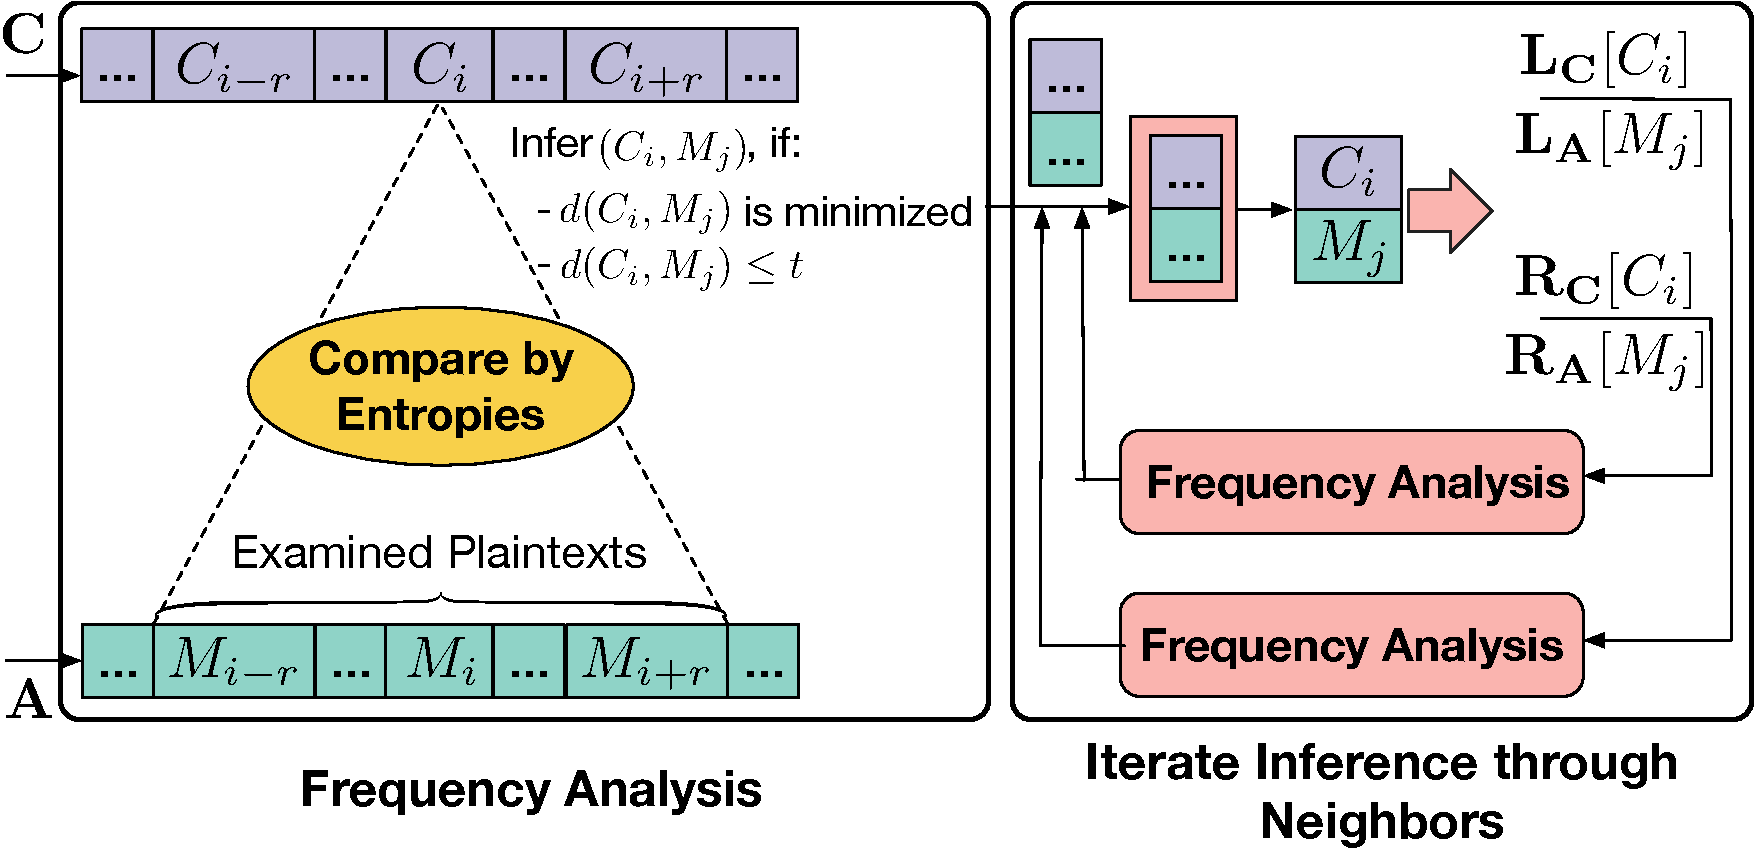
\includegraphics[width=.48\textwidth]{pic/distribution-attack.pdf}
\caption{Workflow of  distribution-based attack.}
\label{fig:distribution-attack}
\end{figure}

Figure \ref{fig:distribution-attack} presents the workflow of the
distribution-based attack. We first sort the unique ciphertexts and  plaintexts by
their frequencies in $\mathbf{C}$ and $\mathbf{A}$, respectively. As in the
locality-based attack \cite{li17}, we configure the parameter $u$ and 
the underlying frequency analysis to return at most $u$ ciphertext-plaintext
pairs.  In particular, for each unique ciphertext $C_i$ of rank $i$ (where 
$1 \leq i \leq u$), we examine a number of unique plaintexts $M_{i-r}, \ldots,
M_i, \ldots, M_{i+r}$ that rank from $i-r$ to $i+r$, where $r$ is a
configurable parameter (e.g., 10 by default) that indicates the maximum range
of rank disturbance that can be addressed. 

For each $C_i$ (where $1\le i\le u$) and the corresponding $M_j$ (where 
$i-r\le j\le i+r$),  we compare their relative frequency distributions by
{\em entropy}, a key concept in information theory that measures the amount of
information produced by a random source. Here, we adopt the entropy to 
{\em quantify the randomness of probability distribution} \cite{wang08}.
Specifically, we define two random variables, denoted by $X$ and $Y$, to
describe the co-occurrences of $C_i$ with its left and right neighbors,
respectively, such that the event ``$X=C$'' denotes the case that $C$ is the
left neighbor of $C_i$, and the event ``$Y=C$'' denotes the case that $C$ is
the right neighbor of $C_i$.  Thus, we compute the probabilities of both
events based on $\mathbf{L_C}$ and $\mathbf{R_C}$:   
%
\begin{eqnarray}
\Pr[X = C] = \frac{\mathbf{L_C}[C_i][C]}{\sum_{C' \in \mathbf{L_C}[C_i]} \mathbf{L_C}[C_i][C']}, \nonumber \\
\Pr[Y = C] = \frac{\mathbf{R_C}[C_i][C]}{\sum_{C' \in \mathbf{R_C}[C_i]} \mathbf{R_C}[C_i][C']}, \nonumber
\end{eqnarray}
%
where $\mathbf{L_C}[C_i]$ and $\mathbf{R_C}[C_i]$ store the left and right
neighbors of $C_i$, respectively, while $\mathbf{L_C}[C_i][C']$ and
$\mathbf{R_C}[C_i][C']$ store the co-occurrence frequencies of $C_i$ with its
left and right neighbor $C'$.  Both $X$ and $Y$ follow the relative frequency
distributions of $C_i$, and we characterize their randomness by entropies
denoted by $e(\mathbf{L_C}[C_i])$ and $e(\mathbf{R_C}[C_i])$, respectively:  
%
\begin{eqnarray}
    e(\mathbf{L_C}[C_i]) = \sum_{C \in \mathbf{L_C}[C_i]} \log_2\frac{1}{\Pr[X = C]}, \nonumber \\
    e(\mathbf{R_C}[C_i]) = \sum_{C \in \mathbf{R_C}[C_i]} \log_2\frac{1}{\Pr[Y = C]}. \nonumber
	% e_{C_i}.r = \sum_{C' \in \mathbf{R_C}[C_i]} {\sf log}_2 \frac{\mathbf{R_C}[C_i][C']}{\sum_{C'' \in \mathbf{R_C}[C_i]} \mathbf{R_C}[C_i][C'']}, 
\end{eqnarray}

Similarly, we compute the entropies $e(\mathbf{L_A}[M_j])$ and
$e(\mathbf{R_A}[M_j])$ of each $M_j$ based on $\mathbf{L_A}$ and
$\mathbf{R_A}$, respectively.  We then quantify the similarity of the relative
frequency distributions of $C_i$ and $M_j$ via the {\em Euclidean distance},
denoted by $d(C_i, M_j)$:  
% is used to measure the amount of information produced by a 
 % random source. Specifically, we compute the entropies $e_{C_i}.l$ and $e_{C_i}.r$ of $C_i$ based on the co-occurrence frequencies of $C_i$ with its left and right neighbors, respectively:  
% \begin{eqnarray}
	% e_{C_i}.l = \sum_{C' \in \mathbf{L_C}[C_i]} {\sf log}_2 \frac{\mathbf{L_C}[C_i][C']}{\sum_{C'' \in \mathbf{L_C}[C_i]} \mathbf{L_C}[C_i][C'']}, \\
	% e_{C_i}.r = \sum_{C' \in \mathbf{R_C}[C_i]} {\sf log}_2 \frac{\mathbf{R_C}[C_i][C']}{\sum_{C'' \in \mathbf{R_C}[C_i]} \mathbf{R_C}[C_i][C'']}, 
% \end{eqnarray}
% where $\mathbf{L_C}[C_i]$ and $\mathbf{R_C}[C_i]$ store the left and right neighbors of $C_i$, respectively, and $\mathbf{L_C}[C_i][C']$ and $\mathbf{R_C}[C_i][C']$ stores the co-occurrence frequencies of $C_i$ with its corresponding neighbor $C'$. Similarly, we compute the entropies $e_{M_j}.l$ and $e_{M_j}.r$ of each $M_j$ based on $\mathbf{L_M}$ and $\mathbf{R_M}$, and collectively measure the similarity of the relative frequency distributions of $C_i$ and $M_j$ via the Euclidean distance:  
\begin{eqnarray*}
	d(C_i, M_j) & = & 
	\big\{[e(\mathbf{L_C}[C_i]) - e(\mathbf{L_A}[M_j])]^2 \\
	& & + \ \ [e(\mathbf{R_C}[C_i]) - e(\mathbf{R_A}[M_j])]^2\big\}^{1/2}.
\end{eqnarray*}

Clearly, $C_i$ and $M_j$ have similar relative frequency distributions only
when the Euclidean distance $d(C_i, M_j)$ of their entropies is small.
Thus,  we identify $(C_i, M_j)$ as an inferred ciphertext-plaintext pair if
they satisfy the following requirements: 
%
\begin{itemize}[leftmargin=*]
\item {\bf R1:} $d(C_i, M_j)$ is the {\em smallest} for all $i-r \leq j \leq i+r$.
\item {\bf R2:} $d(C_i, M_j)$ is not larger than a pre-defined parameter $t$ (e.g., 1 by default).
\end{itemize}

% One special note is R1 is necessarily that some $M_j$  satisfies R1. 

One special note is that the original plaintext of $C_i$ may fall outside of
the examined plaintexts $M_{i-r}, \ldots, M_{i+r}$. 
In this case, R1 is still satisfied by some $M_j$ ($i-r \leq j \leq i+r$), and we expect to filter the incorrect ciphertext-plaintext pair by R2.     



% {\bf We use the requirement R2, and expect it can filter the flawed
% inference results that map $C_i$ to some $M_j$ in this case. PC: don't quite
% understand the statement???}

Then, we adopt the iteration paradigm in the prior locality-based attack \cite{li17} (see Section~\ref{sec:prior-attack}) to increase the coverage of inferred ciphertext-plaintext pairs. Specifically, for each inferred $(C_i, M_j)$, we apply the new frequency analysis scheme (see above) to infer more ciphertext-plaintext pairs through the neighbors of $C_i$ and $M_j$, and further iterate the same inference for those newly inferred pairs. We finally stop the iteration, when none of new ciphertext-plaintext pairs can be inferred.         

% Like the prior attack , we then iterate with each inferred  to infer more ciphertext-plaintext pairs from their neighbors. We apply the proposed new frequency analysis scheme (see above) through the left and right neighbors of $C_i$ and $M_j$, respectively, and      
% through the neighbors of  to infer more . , and further iterate   
% {\bf PC: can we not mention $\mathcal{Q}$ in this paragraph???} Then, we operate a first-in-first-out queue $\mathcal{Q}$, and apply the same locality-based paradigm (see Section~\ref{sec:prior-attack}) like the prior attack \cite{li17}. Specifically, we initialize $\mathcal{Q}$ with all ciphertext-plaintext pairs that have already been inferred. Each time, we pick one pair $(C_i, M_j)$ out of $\mathcal{Q}$, and apply the distribution-based frequency analysis (see above) over the left and right neighbors of $C_i$ and $M_j$, respectively. We include the newly inferred ciphertext-plaintext pairs into $\mathcal{Q}$, and finally stop the iteration until $\mathcal{Q}$ is empty.

 % For each inferred pair $(C_i, M_j)$, we apply the same locality-based paradigm like the prior attack \cite{li17}. Specifically, we operate a first-in-first-out queue $\mathcal{Q}$
% To repeat the distribution-based ranking, we initialize a first-in-first-out queue $\mathcal{Q}$ with the ciphertext-plaintext pairs inferred in Step 1. Each time, we pick one pair $(C_i, M_j)$ out of $\mathcal{Q}$, and apply the distribution-based ranking over their corresponding neighbors $\mathbf{L_C}[C_i]$ and $\mathbf{L_M}[M_j]$, as well as $\mathbf{R_C}[C_i]$ and $\mathbf{R_M}[M_j]$. From each case, we infer new ciphertext-plaintext pairs, and add them into $\mathcal{Q}$ for future loops. We finally stop the loop until $\mathcal{Q}$ is empty.
 % Our rationale of R2 is , and the parameter $t$ helps filter  
 % helps filter out these flawed inference results. 

\subsection{Summary} To summarize, the distribution-based attack provides a
more general notion of locality by considering the relative frequency
distribution during frequency analysis.  It is configured by three parameters
(i) $u$, which specifies the maximum number of ciphertext-plaintext pairs returned by frequency analysis, 
(ii) $r$, which specifies the maximum range of rank disturbance to be
considered, and (iii) $t$, which specifies the Euclidean distance threshold to
filter possibly incorrect inference results. 
The prior locality-based attack \cite{li17} can be regarded as a special case
of the distribution-based attack under the parameter configuration of $r = 0$
(i.e., without addressing any disturbance to frequency ranking) and 
$t\rightarrow\infty$ (i.e., without filtering any incorrect inference results).     
 
 % to 
 % specify the maximum range of disturbance to frequency ranking the scheme considers to address and the maximum entropy threshold  
 
 

% The locality-based attack can be regarded as a special case of the distribution-based attack under the  


\section{Exploiting Size Leakage}

We propose an advanced variant of the distribution-based attack that operates with size information to further reduce false positives. Specifically, we assume that the size of each ciphertext in $\mathbf{C}$ reflects that of its original plaintext.   

% The distribution-based attack addresses the precision of inference results by comparing relative frequency distributions. We argue that there is oppurtunity to further reduce the number of false positives by exploiting size leakage. Specifically, we make an additional assumption that  

% The rationale is symmetric encryption (e.g., block cipher) preserves the number of blocks.

Our idea builds on the fundamental truth that if a ciphertext $C$ corresponds to a plaintext $M$, then the size of $C$ approximates that of $M$. This is because encrypted deduplication preserves the number of blocks (i.e., the basic units operated by symmetric encryption) in the content to be encrypted. We use this fact to further filter the incorrect ciphertext-plaintext pairs $(C, M)$, where the number of blocks in $C$ and $M$ are different.  

% In other words, the number of blocks in each plaintext is exactly mapped to that in the corresponding ciphertext.     

% Our idea is based on the fundamental truth that if $C$ is mapped from $M$, then the size of $C$ approximates that of $M$. This is because encrypted deduplication preserves the number of blocks. In other words, we can filter the candiate pair $(C_i, M_j)$, where the number of blocks of $C_i$ and $M_j$ are different. 

In this work, we assume that each block is of 16 bytes, which is a typical configuration for AES. For each considered ciphertext-plaintext pair $(C_i, M_j)$, we derive the number of blocks in $C_i$ and $M_j$ as $b({C_i})$ and $b({M_j})$, respectively:
\begin{eqnarray*}
b({C_i}) = \lceil \frac{{\sf size}(C_i)}{16} \rceil, \nonumber \\
b({M_j}) = \lceil \frac{{\sf size}(M_j)}{16} \rceil, \nonumber 
\end{eqnarray*}
where ${\sf size}(C_i)$ and ${\sf size}(M_j)$ are the exact sizes of $C_i$ and $M_j$, respecitively, and $\lceil x \rceil$ returns the smallest integer greater than or equal to $x$. In addition to R1 and R2 (see Section~\ref{sec:distribution-attack-description}), we apply the following requirement to filter by size:    
\begin{itemize}[leftmargin=*]
    \item {\bf R3:} $b({C_i})$ equals $b({M_j})$.
\end{itemize}

The requirement R3 is effective to filter the incorrect ciphertext-plaintext pairs regarding variable-size chunks, where different chunks possibly have distinct sizes. However, for fixed-size chunks, it is always satisfied by the ciphertext-plaintext pairs, even they are incorret. Despite of this, we can still apply R1 and R2 to achieve high-precision attack.        



% for filtering false positives in terms of only variable-size chunks, where different chunks have possibly distinct sizes. On the other hand, it is always satisfied by fixed-size chunks, and cannot improve the precision of inference results in this case. Even so, we can still apply R1 and R2 to significantly reduce the amount of false positives in the locality-based attack \cite{li17} (see Section~\ref{sec:distribution-attack-description}).

% by {\bf about 50\%} (see Section~\ref{sec:experiment-distribution}). 

% percentage of false positives below 25\% .       

% \paragraph{Discussion:}
% The filtering effect of R3 depends on the size distribution of  (variable-size) chunks. Since encrypted deduplication only preserves approximate size (i.e., the number of blocks), R3 cannot detect the false positive, which maps a ciphertext to some flawed plaintext that shares the same number of blocks with corresponding exact plaintext. This makes it less effective in addressing inference precision against the workloads, where the sizes of majority chunks are clustered within a small range.   


% Specifically, it is less effective in reducing the number of false positives against the workloads, in which the sizes of chunks are clustered into a small range. The reason is the adversary who observes the size of a ciphertext can only deduce the number of blocks in corresponding plaintext.  


% The plaintexts whose sizes are clustered are more likely to have the same number of blocks, and the adversary cannot distinguish them by size.   


% The main reason is the adversary can deduce the size of the plaintext in the quantization factor of block size.   
% Due to the above facts, an adversary who can see the length of a ciphertext can readily deduce the length of the respective plaintext, except for a quantization factor of 8 or 128 respectively. The larger the quantization factor, the less resolution the attacker has regarding plaintext length information. Rupture is able to attack ciphers with even large quantization factors, yet a larger factor can make the attack slower. While the quantization factor can be made arbitrarily large when designing ciphers, the penalty being paid is in bandwidth consumed to transmit the ciphertext.
% and R3 is less effective in reducing the false positives against small-size chunks.
% only for variable-size chunks, where different chunks have possibly distinct sizes. It is naturally satisfied by fixed-size chunks, and cannot filter any false positives. In this case, this  
% In addition, the effect of R3 depends on the (average) size of chunks.  



% \paragraph{Discussion:}
% The size-based attack builds on the assumption of varying sizes of chunks, and demonstrates security alert only in variable-size chunking. In other words, the size-based attack will degrade to classical frequency analysis under fixed-size chunking, in which all plaintexts or ciphertexts have a uniform size and come into a single entry of the associative array.  
% The effectiveness of the size-based attack depends on the (average) size of chunks, and it is less effective for inferring small-size chunks. For example, we have evaluated that the size-based attack infers as low as 0.32\% of ciphertext-plaintext pairs against the chunks of an average size of 2KB (for comparison, it can infer up to 31.3\% ciphertext-plaintext pairs in our experiment of 8KB-size chunks, see Section~\ref{sec:experiment-size}). This is mainly for two reasons. First, small-size chunks are likely to have limited  variance on their size, and aggregate into a few entries of the associative array; this degrades the coverage of inferred pairs (recall that the attack  returns a limited number of ciphertext-plaintext pairs for each available chunk size). Second, each entry of the associative array is likely to include a large amount of small-size chunks, among which
% there tend to exist many ties where chunks have the same frequency; 
 % this possibly introduces additional false positives into frequency analysis \cite{naveed15, li17}. 




% For each $M_j$ ($i-r \leq j \leq i+r$), we compute similar entropies $e_{M_j}.l$ and $e_{M_j}.r$ for $M_j$, and collectively measure the similarity of the relative frequency distributions of $C_i$ and $M_j$ via the Euclidean distance:  

% We first sort available ciphertexts and plaintexts by their frequencies in $\mathbf{C}$ and $\mathbf{M}$, respectively. Next, we consider the distribution-based ranking scheme configured by a tuple of parameters $(u, r, t)$, in order to infer at most $u$ ciphertext-plaintext pairs. Specifically, for each ciphertext $C_i$ of rank $i$ ($1 \leq i \leq u$), we examine the plaintexts $M_{i-r},\ldots,M_i,\ldots,M_{i+r}$ that rank from $i-r$ to $i+r$, where $r$ (e.g., 10 by default) indicates the maximum range of rank disturbance can be addressed by the distribution-based ranking scheme. Then, we compute the entropies $e_{C_i}.l$ and $e_{C_i}.r$ of $C_i$ based on the co-occurrences of $C_i$ with its left and right neighbors, respectively:\footnote{Alternatively, we can calculate the entropies (that depend on the associative arrays $\mathbf{L_C}$ and $\mathbf{R_C}$) in
% pre-processing, rather than computing them on the fly.} 
% \begin{eqnarray}
% 	e_{C_i}.l = \sum_{C' \in \mathbf{L_C}[C_i]} {\sf log}_2 \frac{\mathbf{L_C}[C_i][C']}{\sum_{C'' \in \mathbf{L_C}[C_i]} \mathbf{L_C}[C_i][C'']}, \\
% 	e_{C_i}.r = \sum_{C' \in \mathbf{R_C}[C_i]} {\sf log}_2 \frac{\mathbf{R_C}[C_i][C']}{\sum_{C'' \in \mathbf{R_C}[C_i]} \mathbf{R_C}[C_i][C'']}, 
% \end{eqnarray}
% where $\mathbf{L_C}[C_i]$ and $\mathbf{R_C}[C_i]$) store the left and right neighbors of $C_i$, respectively, and $\mathbf{L_C}[C_i][C']$ and $\mathbf{R_C}[C_i][C']$ stores the co-occurrences of $C_i$ with its corresponding neighbor $C'$. For each $M_j$ ($i-r \leq j \leq i+r$), we compute similar entropies $e_{M_j}.l$ and $e_{M_j}.r$ for $M_j$, and collectively measure the similarity of the relative frequency distributions of $C_i$ and $M_j$ via the Euclidean distance:  
% \begin{eqnarray}
% 	{\sf Sim}(C_i, M_j) = \sqrt{(e_{C_i}.l - e_{M_j}.l)^2 + (e_{C_i}.r - e_{M_j}.r)^2}.  
% \end{eqnarray}

%  We infer $(C_i, M_j)$ as a ciphertext-plaintext pair, if (i) ${\sf Sim}(C_i, M_j)$ is the {\em smallest} among all examined plaintexts, and (ii) ${\sf Sim}(C_i, M_j)$ is not larger than the parameter $t$ (e.g., 1 by default). Our rationale is that the original plaintext of $C_i$ may fall outside of $M_{i-r}, \ldots, M_{i+r}$ (e.g., the range of rank disturbance is greater than $r$), and the pre-defined upper bound $t$ helps filter out these flawed inference results. 





% Our insight is that if $M$ is the underlying plaintext of $C$, then the relative frequency distributions of $C$ and $M$ are likely to be {\em similar}. The rationale is that $\mathbf{M}$ and $\mathbf{C}$ are from the same primary data (at different time), and hence share a large stretch of unchanged chunks due to chunk locality. Thus, we can adjust the ranking of classical frequency analysis by taking relative frequency distribution into consideration. Specifically, for each ciphertext $C_i$ of rank $i$ and plaintext $M_j$ of rank $j$, we compare their relative frequency distributions, say by the {\em entropies} on the co-occurrences of their neighbors. If they have similar entropy values, we say their relative frequency distributions are similar, and we call $(C_i, M_j)$ as an inferred ciphertext-plaintext pair, even though $C_i$ and $M_j$ have different ranks (i.e., $i \neq j$). 



% Thus, we can operate frequency analysis while taking relative frequency distribution into consideration, in order to filter out the inference results, in which the relative frequency distributions of the ciphertext and plaintext are significantly different. 
% Specifically, for each  plaintext $M$, we consider its {\em relative frequency distribution} that is counted by the co-occurrences of $M$ with its neighboring plaintexts (recall that $M$ may have duplicate copies and hence multiple neighbors in $\mathbf{M}$). We also count the relative frequency distribution of each ciphertext $C$.  
 % Thus, we can adjust the ranking of classical frequency analysis by taking relative frequency distribution into consideration. Specifically, for each ciphertext $C_i$ of rank $i$ and plaintext $M_j$ of rank $j$, we compare their relative frequency distributions, say by the {\em entropies} on the co-occurrences of their neighbors. If they have similar entropy values, we say their relative frequency distributions are similar, and we call $(C_i, M_j)$ as an inferred ciphertext-plaintext pair, even though $C_i$ and $M_j$ have different ranks (i.e., $i \neq j$). 
% The key idea of our attack is to inspect the distribution of , so as to filter out potentially flawed inference results.
% t further inspects the relative frequency distribution of the data and filters any potentially flawed inference results.
% We propose to extend chunk locality, and examine the frequency .  




% Inspired by chunk locality (see \S\ref{sec:locality}), we move one step further to examine the co-occurrence of neighboring chunks.
% Specifically, for each chunk, we consider its {\em relative frequency distribution} that is counted by the number of co-occurrences with its neighbors (recall that a chunk may have duplicate copies and hence multiple neighboring chunks). Our insight is that identical chunks likely have {\em similar} relative frequency distributions across backups. The rationale is updates to backups appear in few clustered regions of chunks, while the remaining majority regions of chunks preserve their co-occurrence relationships.


% Chunk locality states that neighboring chunks tend to co-occur under the same order across backups. For example, if a plaintext $M$ is surrounded by the plaintexts $M'$ and $M''$ in one backup, then $M$ is also likely to be surrounded by $M'$ and $M''$ in the following backups. Prior works \cite{xia11,lillibridge09,zhu08} have exploited chunk locality to improve performance, while we adapt it into addressing the false positives in frequency analysis. Specifically, classical frequency analysis is sensitive to frequency ranking, and any disturbances (e.g., due to data updates across backups or ranking the ciphertexts/plaintexts that have identical frequency) to the frequency ranking can introduce a significant amount of flawed inference results.  
   % In the following, we show how to build on chunk locality to construct an inference attack with low false positives. We first elaborate the key designs of the distribution-based attack, and then present the attack details step by step. 


% {\bf say drawback of classical frequency analysis}   

   


% Take {\em backups}, the complete copies of some primary data (e.g., application states, file systems, and VM images), as an example, if a plaintext $M$ is surrounded by the plaintexts $M'$ and $M''$ in one backup, then $M$ is also likely to be surrounded by $M'$ and $M''$ in the following backup from the same primary data. Prior works \cite{xia11,lillibridge09,zhu08} have exploited chunk locality to improve performance, while we adapt it into addressing the false positives of inference attack.   

% Figure \ref{fig:distribution-attack} shows an overview of the distribution-based attack. Given the input of $\mathbf{M}$ and $\mathbf{C}$, it builds on the {\em distribution-based ranking} to reduce the number of false positives in classical frequency analysis. Specifically, for each  plaintext $M$, we consider its {\em relative frequency distribution} that is counted by the co-occurrences of $M$ with its neighboring plaintexts (recall that $M$ may have duplicate copies and hence multiple neighbors in $\mathbf{M}$). We also count the relative frequency distribution of each ciphertext $C$.  
% Our insight is that if $M$ is the underlying plaintext of $C$, then the relative frequency distributions of $C$ and $M$ are likely to be {\em similar}. The rationale is that $\mathbf{M}$ and $\mathbf{C}$ are from the same primary data (at different time), and hence share a large stretch of unchanged chunks due to chunk locality. Thus, we can adjust the ranking of classical frequency analysis by taking relative frequency distribution into consideration. Specifically, for each ciphertext $C_i$ of rank $i$ and plaintext $M_j$ of rank $j$, we compare their relative frequency distributions, say by the {\em entropies} on the co-occurrences of their neighbors. If they have similar entropy values, we say their relative frequency distributions are similar, and we call $(C_i, M_j)$ as an inferred ciphertext-plaintext pair, even though $C_i$ and $M_j$ have different ranks (i.e., $i \neq j$). 

% For each inferred ciphertext-plaintext pair $(C_i, M_j)$, we repeat the same inference (see above) through their neighbors. Specifically, we collect the left and right neighbors of $C_i$,  as well as of $M_j$, respectively, and apply the distribution-based ranking over their corresponding neighbors, in order to infer new ciphertext-plaintext pairs. The rationale is that chunk locality preserves orders, and the left and right neighbors of $M_j$ are likely to be the underlying plaintexts of the left and right neighbors of $C_i$, respectively. We further repeat the inference through the neighbors of these newly inferred ciphertext-plaintext pairs, so as to increase the coverage of inferred pairs.  

% Then, we describe the details of the distribution-based attack.


% The distribution-based ranking proceeds as follows. We first rank available ciphertexts and plaintexts by their frequencies in $\mathbf{C}$ and $\mathbf{M}$, respectively. 
% Thus, we can adjust the ranking of classical frequency analysis by taking the relative frequency distribution of each plaintext and ciphertext into account. In other words, suppose $C_i$ and $M_j$ are the $i$-th and $j$-th top frequent ciphertext and plaintext, respectively.  
% This allows to infer the ciphertext-plaintext pair like $(C_i, M_j)$ 
% To perform distribution-based ranking, 



% Thus, we          
% Thus, we first establish the frequency-only ranking like classical frequency analysis (see \S\ref{sec:freqanalysis}), and then adjust the ranking by taking into account the relative frequency distributions of chunks. Roughly, we break rank disturbances and infer the ciphertext-plaintext chunks pairs
% $(C_i, M_j)$, where $C_i$ and $M_j$ have similar relative frequency distribution yet possibly different ranks (e.g., $i \neq j$). We refer the Step 1 of the attack for detailed requirements of $C_i$ and $M_j$.  



% We propose a new (frequency-based) ranking primitive, named {\em distribution-based ranking}, to address the ties incurred in classcial frequency analysis (see \S\ref{sec:freqanalysis}). Specifically, for each chunk, we consider its {\em relative frequency distribution} that is counted by the co-occurrences with its neighbors (recall that a chunk may have duplicate copies and hence multiple neighbors). Our insight is that the relative frequency distribution of the same chunk must be similar across backups. The reason is chunk locality implies that the majority stretches of chunks are unchanged. Thus, we first establish the frequency-only ranking like classical frequency analysis (see \S\ref{sec:freqanalysis}), and then adjust the ranking by taking into account the relative frequency distributions of chunks. Roughly, we break rank disturbances and infer the ciphertext-plaintext chunks pairs
% $(C_i, M_j)$, where $C_i$ and $M_j$ have similar relative frequency distribution yet possibly different ranks (e.g., $i \neq j$). We refer the Step 1 of the attack for detailed requirements of $C_i$ and $M_j$.  
% We elaborate the details below.

% \paragraph{Step 1 (Distribution-based ranking):}
% We first sort available ciphertexts and plaintexts by their frequencies in $\mathbf{C}$ and $\mathbf{M}$, respectively. Next, we consider the distribution-based ranking scheme configured by a tuple of parameters $(u, r, t)$, in order to infer at most $u$ ciphertext-plaintext pairs. Specifically, for each ciphertext $C_i$ of rank $i$ ($1 \leq i \leq u$), we examine the plaintexts $M_{i-r},\ldots,M_i,\ldots,M_{i+r}$ that rank from $i-r$ to $i+r$, where $r$ (e.g., 10 by default) indicates the maximum range of rank disturbance can be addressed by the distribution-based ranking scheme. Then, we compute the entropies $e_{C_i}.l$ and $e_{C_i}.r$ of $C_i$ based on the co-occurrences of $C_i$ with its left and right neighbors, respectively:\footnote{Alternatively, we can calculate the entropies (that depend on the associative arrays $\mathbf{L_C}$ and $\mathbf{R_C}$) in
% pre-processing, rather than computing them on the fly.} 
% \begin{eqnarray}
% 	e_{C_i}.l = \sum_{C' \in \mathbf{L_C}[C_i]} {\sf log}_2 \frac{\mathbf{L_C}[C_i][C']}{\sum_{C'' \in \mathbf{L_C}[C_i]} \mathbf{L_C}[C_i][C'']}, \\
% 	e_{C_i}.r = \sum_{C' \in \mathbf{R_C}[C_i]} {\sf log}_2 \frac{\mathbf{R_C}[C_i][C']}{\sum_{C'' \in \mathbf{R_C}[C_i]} \mathbf{R_C}[C_i][C'']}, 
% \end{eqnarray}
% where $\mathbf{L_C}[C_i]$ and $\mathbf{R_C}[C_i]$) store the left and right neighbors of $C_i$, respectively, and $\mathbf{L_C}[C_i][C']$ and $\mathbf{R_C}[C_i][C']$ stores the co-occurrences of $C_i$ with its corresponding neighbor $C'$. For each $M_j$ ($i-r \leq j \leq i+r$), we compute similar entropies $e_{M_j}.l$ and $e_{M_j}.r$ for $M_j$, and collectively measure the similarity of the relative frequency distributions of $C_i$ and $M_j$ via the Euclidean distance:  
% \begin{eqnarray}
% 	{\sf Sim}(C_i, M_j) = \sqrt{(e_{C_i}.l - e_{M_j}.l)^2 + (e_{C_i}.r - e_{M_j}.r)^2}.  
% \end{eqnarray}

%  We infer $(C_i, M_j)$ as a ciphertext-plaintext pair, if (i) ${\sf Sim}(C_i, M_j)$ is the {\em smallest} among all examined plaintexts, and (ii) ${\sf Sim}(C_i, M_j)$ is not larger than the parameter $t$ (e.g., 1 by default). Our rationale is that the original plaintext of $C_i$ may fall outside of $M_{i-r}, \ldots, M_{i+r}$ (e.g., the range of rank disturbance is greater than $r$), and the pre-defined upper bound $t$ helps filter out these flawed inference results. 


% We  apply classical frequency analysis to establish the (frequency-only) ranking on the plaintext chunks in $\mathbf{M}_{\rm a}$, as well as on the ciphertext chunks in $\mathcal{L}_{\rm order}$. Like the size-based attack (see \S\ref{sec:size-attack-description}), we configure the parameter $u$ that indicates the {\em maximum} number of most frequent chunk pairs to be inferred by our distribution-based ranking scheme.  
% Then,  For $C_i$ and each $M_j$ $(i-r \leq j \leq i+r)$, we compare their relative frequency distributions, say by the {\em entropies} of neighboring chunks. Specifically, we compute the entropies $e_{M_j}.l$ and $e_{M_j}.r$ based on the co-occurrences of $M_j$ and its left and right neighbors, respectively:    
% (recall that we can access the co-occurrences of $M_j$ and its neighbors from $\mathbf{L}_{\rm a}$ and $\mathbf{R}_{\rm a}$).    



% For example, if a chunk $M$ is surrounded by the chunks $M'$ and $M''$ in one backup, then $M$ is also likely to be surrounded by $M'$ and $M''$ in the following backups. The rationale is that the changes of backups often affect a few chunks, while the remaining chunks repeat in the same order. 

% The distribution-based attack builds on {\em chunk locality}  that is defined based on the neighborhood of chunks. Specifically, given a logical chunk $M^{\langle i \rangle}$, we define its {\em left} (resp. {\em right}) {\em neighbor} as the logical chunk $M^{\langle i-1 \rangle}$ (resp. $M^{\langle i+1 \rangle}$) that appears directly before (resp. after) $M^{\langle i \rangle}$. 

% To capture chunk locality, we build the associative arrays $\mathbf{L}_{\rm a}$ and $\mathbf{R}_{\rm a}$, which store the co-occurrences of neighboring  chunks in the auxiliary information $\mathbf{M}_{\rm a}$. Specifically, for two neighboring chunks $M$ and $M'$, $\mathbf{L}_{\rm a}[M][M']$ (resp. $\mathbf{R}_{\rm a}[M][M']$) stores the number of times that $M'$ is the left (resp. right) neighbor of $M$. For the ciphertext chunks, we also extract $\mathbf{L}_{\rm t}$ and $\mathbf{R}_{\rm t}$ to store the co-occurrences of their original chunks (recall that we can access the orders of original chunks by $\mathcal{L}_{\rm order}$).

% even they have different frequency ranks of $i$ and $j$ (see Step 1 for detailed requirements on .    
% This allows us to address rank disturbances and infer the 

% We propose the {\em distribution-based ranking}, which exploits the co-occurrences of neighboring chunks to address the rank disturbances (e.g., due to data updates or breaking ties) of classical frequency analysis (\S\ref{sec:freqanalysis}). Specifically, for each chunk,   



% the distribution-based ranking through their neighboring chunks. Specifically, we establish the distribution-based ranking on the left and right neighbors of $C_i$ and $M_j$, and infer more ciphertext-plaintext chunk pairs. The rationale is that the neighbors of $M_j$ are likely to be the neighbors of the original chunk of $C_i$, since chunk locality implies that the orders of chunks are preserved. We iterate the similar inference through the neighbors of those newly inferred chunk pairs, so as to increase attack severity.  

    
% Thus, we can infer more ciphertext-plaintext chunk pairs and increase attack severity based on the iterative inferences. 



% In this work,  a tuple $(u, r, t)$ of parameters.
% the co-occurrences of neighboring chunks are likely to be preserved across backups. 


% (recall that we can access the logical orders of original chunks from $\mathcal{L}_{\rm order}$). 
% Based on the data structures, we first propose a new frequency analysis primitive, the {\em distribution-based ranking}, to address the rank disturbances of classical frequency analysis (\S\ref{sec:freqanalysis}). Then, we explain how to exploit chunk locality to repeat the inference primitive for high severity.   
% introduce a building block,  of the attack, followed by how to repeat the inference for high severity.      
% \paragraph{Distribution-based ranking:}
% Frequency analysis is sensitive to frequency ranking, and any disturbances (e.g., due to data updates or breaking ties) to the ranks can greatly degrade its inference accuracy. Inspired by chunk locality, we propose to examine the  
% updates to backups commonly appear in few clustered regions of chunks, while the remaining majority  chunks preserve their co-occurrence relationships.


% \paragraph{Step 2 (Repeat distribution-based ranking through neighbors):}
% To repeat the distribution-based ranking, we initialize a first-in-first-out queue $\mathcal{Q}$ with the ciphertext-plaintext pairs inferred in Step 1. Each time, we pick one pair $(C_i, M_j)$ out of $\mathcal{Q}$, and apply the distribution-based ranking over their corresponding neighbors $\mathbf{L_C}[C_i]$ and $\mathbf{L_M}[M_j]$, as well as $\mathbf{R_C}[C_i]$ and $\mathbf{R_M}[M_j]$. From each case, we infer new ciphertext-plaintext pairs, and add them into $\mathcal{Q}$ for future loops. We finally stop the loop until $\mathcal{Q}$ is empty.


% For each inferred chunk pair $(C_i, M_j)$, we build the {\em locality-based loop} \cite{li17} to repeat inferences through their neighboring chunks. Specifically, we collect the set of left $\mathbf{L}_{\rm t}[C_i] = \{C': \mathbf{L}_{\rm t}[C_i][C'] > 0 \}$ and right $\mathbf{R}_{\rm t}[C_i] = \{C': \mathbf{R}_{\rm t}[C_i][C'] > 0 \}$ neighbors of $C_i$, as well as the left $\mathbf{L}_{\rm a}[M_j]$ and right $\mathbf{R}_{\rm a}[M_j]$ neighbors of $M_j$. Then, we establish the distribution-based ranking over the chunks in $\mathbf{L}_{\rm t}[C_i]$ and $\mathbf{L}_{\rm a}[M_j]$, as well as in $\mathbf{R}_{\rm t}[C_i]$ and $\mathbf{R}_{\rm a}[M_j]$, respectively, so as to infer more ciphertext-plaintext chunk pairs. The rationale is that the chunks in $\mathbf{L}_{\rm a}[M_j]$ (resp. $\mathbf{R}_{\rm a}[M_j]$) are likely to be the underlying
% plaintexts of the ciphertext chunks in $\mathbf{L}_{\rm t}[C_i]$ (resp. $\mathbf{R}_{\rm t}[C_i]$), since chunk locality implies that the orders of chunks are preserved. We further iterate the similar inference through the neighbors of those newly inferred chunk pairs, so as to increase attack severity.     
 % In other words, we infer the ciphertext-plaintext chunk pairs, say $(C, M)$, from the neighbors of $C_i$ and $M_j$, such that (i) $C$ and $M$ have the most co-occurrences with $C_i$ and $M_j$, respectively and (ii) the relative frequency distributions of $C$ and $M$ are highly similar. We add the newly inferred  chunk pairs into $\mathcal{Q}$, and finally stop the loop until $\mathcal{Q}$ is empty.



% A special note is that we only examine the possible plaintext chunks that rank from $i$ to $i+r$ (rather than $i-r$ to $i+r$) for the distribution-based ranking in the loop. Our rationale is that chunks may have low co-occurrences after a number of loops, and most of them are likely to have similar relative frequency distribution with $C_i$. We start examination from rank $i$ to avoid relating the plaintext chunk that has a large rank difference from $i$.  

% and all inferred chunk pairs have been iterated. 


% and identify their neighbor sets $\mathbf{L}_{\rm t}[C_i], \mathbf{R}_{\rm t}[C_i], \mathbf{L}_{\rm a}[M_j]$ and $\mathbf{R}_{\rm a}[M_j]$. We invoke the distribution-based ranking on $\mathbf{L}_{\rm t}[C_i]$ and $\mathbf{L}_{\rm a}[M_j]$, as well as on $\mathbf{R}_{\rm t}[C_i]$ and $\mathbf{R}_{\rm a}[M_j]$, and add the newly inferred ciphertext-plaintext chunk pairs into $\mathcal{Q}$. 





% Specifically, the adversary first applies frequency analysis to initialize an inferred set $\mathcal{G}$ with a configurable number (parameterized by $u$) of top-frequent ciphertext-plaintext chunk pairs. These inferred pairs can be considered correct with a high probability when $u$ is not much large (see \S\ref{sec:bucket_description}). In each iteration, the adversary picks one pair $(C, M)$ out of $\mathcal{G}$, and identifies the corresponding neighboring chunks $\mathbf{L}_\mathcal{C}[C]$, $\mathbf{R}_\mathcal{C}[C]$, $\mathbf{L}_\mathcal{M}[M]$ and $\mathbf{R}_\mathcal{M}[M]$ of $C$ and $M$. It applies frequency analysis on $\mathbf{L}_\mathcal{C}[C]$ and $\mathcal{L}_\mathcal{M}[M]$, as well as $\mathbf{R}_\mathcal{C}[C]$ and $\mathbf{R}_\mathcal{M}[M]$, according to their co-occurrence frequencies with $C$ and $M$. The rationale is the order of chunks is preserved due to locality, and the left and right neighbors of $M$ are likely to be the original chunks of the left and right neighbors of $C$. The adversary adds the newly inferred top-frequent chunk pairs into $\mathcal{G}$, and iterates until $\mathcal{G}$ is empty.  
% from $\mathbf{L}_{\rm t}$ and $\mathbf{R}_{\rm t}$.   
% since a chunk may have duplicate copies and hence multiple neighbors, we :w
% can compute the entropies $\mathbf{E}_{\rm tar}[C_i].l$ and $\mathbf{E}_{\rm tar}[C_i].r$, as well as $\mathbf{E}_{\rm aux}[M_j].l$ and $\mathbf{E}_{\rm aux}[M_j].r$, based on the co-occurrences of the neighbors of $C_i$ and $M_j$. Thus, we can collectively measure the similarity of relative frequency distributions via Euclidean distance: 
% Note that our ranking approach combines the co-occurrence relationship of neighboring chunks to address the rank disturbance of frequency-only ranking. It does not require each inferred pair $(C_i, M_j)$ must have the same rank, i.e., $j$ does not need to equal $i$.  In \S\ref{}, we will experimentally justify its advantage in distribution-based attack (\S\ref{sec:distribution-description}).   
% Based on chunk locality, we 

% \subsection{Discussion}
% \label{sec:distribution-discussion}

% \noindent {\bf Generalization of prior attack:} 
% The recent {\em locality-based attack} \cite{li17} builds on chunk locality as our work, in order to improve the severity of frequency analysis against encrypted deduplication. The main difference is the prior attack \cite{li17} uses classical frequency analysis as the inference primitive (used in both Step 1 and Step 2 in Section~\ref{sec:distribution-attack-description}), rather than applying the distribution-based ranking to filter out flawed inference results. In fact, it \cite{li17} can be regarded as a special case of the distribution-based attack under the parameter configuration of $r = 0$ (i.e., cannot address rank disturbances) and $t = \infty$ (i.e., cannot filter out any flawed inference results). 

% \paragraph{Fine-grained ordering knowledge:}
% For each ciphertext, the distribution-based attack assumes that its deduplication processing sequence reflects the logical order of corresponding plaintext, so that the adversary can identify the neighboring ciphertexts for attack. The assumption holds in a variety of real-world storage systems \cite{xia11,lillibridge09,zhu08} that preserve orders in deduplication, yet it can be addressed by scrambling the orders of ciphertexts. 
% % This breaks their neighborhood relationships, and hence prevents the attack.  


% (see \S\ref{sec:countermeasure}    


% To launch the distribution-based attack, the adversary must have the order information of ciphertexts. In other words, for each ciphertext, the attack  
% Although the assumption is plausible in a variety ,  
% the orders of ciphertexts reflect the  
% knows the logical order of underlying plaintexts in priori. 

% The distribution-based attack has some limitations. First, the attack assumes that the adversary has full knowledge of neighboring chunks. Although it is plausible for some deduplicaton systems \cite{xia11,lillibridge09,zhu08}, we can address the assumption by simply swapping the orders of chunks (see \S\ref{sec:countermeasure}). Second, the attack depends on the prevalence of locality in workloads, and it may perform poor in the low-locality workloads. 

% In Section~\ref{sec:experiment-distribution}, we will experimentally show that our new attack 
% can significantly reducing the number of false positives.



% it is reasonable to replace the frequency-only ranking (in classical frequency analysis) by our generalized distribution-based ranking. The reason is the inference precision of classical frequency analysis is strongly susceptible to rank disturbances. 
 % Any incorrectly inferred ciphertext-plaintext chunk pairs will compromise the following inference loops over their neighbors, and  affect inference rate. In \S\ref{sec:experiment-distribution}, we experimentally examine the improvement of our distribution-based attack over the prior locality-based attack \cite{li17}.
 % , which builds on classical frequency analysis as the underlying primitive.    
% repeat inferences .     
% Like the , the  builds on the same characteristics of  to demonstrate the security vulnerability of encrypted deduplication.
% Recently, Li {\em et al.}  , which builds on chunk locality as the distribution-based attack. The difference is the   
% repeats classical frequency analysis through neighbors of each inferred ciphertext-plaintext pair. 


% This limits the adaptability of the distribution-based attack. %for the low-locality workloads (\S\ref{sec:clustering-attack}).
%, in which the data chunks arrive in the server under random order or from disparate clients.    

% % We first review the {\em locality-based attack} \cite{li17} 
% % that combines frequency and order information to infer plaintext content in encrypted deduplication. Then, we present {\em distribution-based attack} that augments the locality-based attack with high inference accuracy. 
% % Note that we do not explicitly exploit size information in these attacks, since they are adapt to fixed-size chunking setting. 

% \subsection{Prior Work: Locality-based Attack}
% \label{sec:locality-attack}
% The locality-based attack \cite{li17} targets backup workloads. It models a prior backup as $\mathbf{M}_{\rm aux}$, and aims to recover the original chunks of a later backup (known as $\mathbf{M}_{\rm tar}$). It builds on {\em chunk locality} \cite{xia11,zhu08}, which specifies that neighboring chunks tend to co-occur again in the same order. The attack defines the {\em left (resp. right) neighbor} of a chunk $M$ is the chunk that appears directly before (resp. after) $M$ in logical order. It derives a key insight that if $M$ is the original chunk of a ciphertext chunk $C$, then the neighbors of $M$ are likely to be the original chunks of the corresponding neighbors of $C$. 

% To represent neighboring relations, the attack assumes that the adversary's knowledge of order information is in the form of the associative arrays $\mathbf{L}_{\rm tar}$ and $\mathbf{R}_{\rm tar}$. Specifically, $\mathbf{L}_{\rm tar}[C]$ (resp. $\mathbf{R}_{\rm tar}[C]$) maps a ciphertext chunk $C$ to its left (resp. right) neighbors and the corresponding co-occurrences with $C$. Note that this can be computed exactly if the adversary knows $\mathcal{L}_{\rm order}$. In addition, the attack extracts similar arrays $\mathbf{L}_{\rm aux}$ and $\mathbf{R}_{\rm aux}$  from $\mathbf{M}_{\rm aux}$.

    



% % which map each ciphertext chunk $C$ to its left and right neighboring chunks and corresponding co-occurrence frequencies with $C$. 


% To launch attack, the adversary iterates frequency analysis to infer the neighbors of each known ciphertext-plaintext chunk pair. Specifically, it first initializes an inferred set $\mathcal{G}$ with a configurable number (e.g., $u$) of top-frequent chunk pairs. In each iteration, it picks one pair $(C, M)$ out of $\mathcal{G}$, and applies frequency analysis on their neighbors $\mathbf{L}_{\rm tar}[C]$ and $\mathbf{L}_{\rm aux}[M]$, as well as $\mathbf{R}_{\rm tar}[C]$ and $\mathbf{R}_{\rm aux}[M]$, and further adds the newly inferred top-frequent chunk pairs into $\mathcal{G}$. The adversary iterates the above procedure until $\mathcal{G}$ is empty.   




%  % and identifies the corresponding neighboring chunks $\mathbf{L}_\mathcal{C}[C]$, $\mathbf{R}_\mathcal{C}[C]$, $\mathbf{L}_\mathcal{M}[M]$ and $\mathbf{R}_\mathcal{M}[M]$ of $C$ and $M$. It applies frequency analysis on $\mathbf{L}_\mathcal{C}[C]$ and $\mathcal{L}_\mathcal{M}[M]$, as well as $\mathbf{R}_\mathcal{C}[C]$ and $\mathbf{R}_\mathcal{M}[M]$, according to their co-occurrence frequencies with $C$ and $M$. The rationale is the order of chunks is preserved due to locality, and the left and right neighbors of $M$ are likely to be the original chunks of the left and right neighbors of $C$.   

  



% % finds the corresponding sets $\mathbf{L_C}[C]$, $\mathbf{L_M}[M]$, $\mathbf{R_C}[C]$ and $\mathbf{R_M}[M]$ of neighboring chunks, and applies frequency analysis on $\mathbf{L_C}[C]$ and $\mathbf{L_M}[M]$, and similarly on $\mathbf{R_C}[C]$ and $\mathbf{R_M}[M]$. 


% % initializes  (e.g., by frequency analysis). The rationale is the frequency ranks of these top-frequent chunks are stable across backups, and hence the inferred pairs are correct with a high probability. 


% % More formally, the adversary knows the following information: $\mathbf{F}_\mathcal{C} = \{ (C, {\sf cnt}(M)) : C \in \mathcal{C} \wedge (M, C) \in \mathcal{E} \}$, which maps each ciphertext chunk to the frequency of its original chunk in $\mathbf{M}_t$, as well as $\mathbf{L}_\mathcal{C} = $ and $\mathbf{R}_\mathcal{C}$ which map each ciphertext chunk to its left and right neighboring chunks and their co-occurrence frequencies, respectively. The adversary also knows the similar associative arrays $\mathbf{F}_\mathcal{M}$, $\mathbf{L}_\mathcal{M}$ and $\mathbf{R}_\mathcal{M}$ about $\mathbf{M}_a$.  

    


% Our observation is that the underlying frequency analysis is {\em sensitive to frequency ranking}. Specifically, any disturbance (e.g., due to data updates or breaking ties) to the frequency rank can greatly degrade inference accuracy. Any incorrectly inferred chunk pairs will further compromise the following iterations of their neighbors, and hence affect inference rate. The original construction \cite{li17} builds on parameter-aware frequency analysis to strengthen accuracy, yet this primitive sacrifices inference coverage as discussed in \S\ref{sec:bucket-description}. 

% % Thus, the attack of \cite{li17}, while valuable for alerting the vulnerabilities of encrypted deduplication, is fairly severe in practice.


% % {\bf The authors \cite{li17} employ parameters to indicate only a small number of top-frequent chunk pairs to be returned by frequency analysis}. However, as discussed in \S\ref{sec:bucket-description}, this trick incurs new problem: a lower bound limits the coverage of inferred chunks, while a higher bound .     

% We argue that there is an opportunity to increase attack severity by extensively exploiting the knowledge of order information. Our view is to build robust frequency ranking for being resistant to rank disturbance. In this way, we can properly increase frequency analysis parameter to infer more chunks, while mitigating the rank disturbance of the relatively non-top chunks to preserve accuracy. In the following two sections, we will elaborate our ranking approach (\S\ref{sec:distribution-ranking}), followed by how to build on it for inference attack (\S\ref{sec:distribution-description}).

  

% % augment the parameter-aware frequency analysis with {\em robust ranking}. This allows to increase the frequency analysis parameter to potentially infer more chunks, while it can mitigate the rank disturbance of relatively non-top chunks to preserve accuracy.





	
% % In \S\ref{sec:distribution_attack_description}, we present a simple but effective approach to establish {\em robust} frequency ranking, so as to ensure the inference accuracy of frequency analysis. We also integrate our approach with the locality-based attack for both severity and accuracy.   

% \subsection{Robust Ranking}
% \label{sec:distribution-ranking}




% \subsection{Attack Description}
% \label{sec:distribution-description}
% % Our view is to build {\em robust} frequency ranking for being resistant to disturbance. In the following, we first propose a robust ranking approach for frequency analysis. Then, we present the {\em distribution-based attack} that augments the prior locality-based attack \cite{li17} with robust frequency ranking for high severity.  

% We now proceed the {\em distribution-based attack}, which replaces the frequency-only ranking of the locality-based attack \cite{li17} by our robust ranking scheme (\S\ref{sec:distribution-ranking}). Algorithm \ref{alg:distribution-attack} shows the attack details. It takes input the frequency analysis parameter $u$, (expected) rank disturbance range $r$, distance threshold $t$, order leakage $\mathcal{L}_{\rm order}$ and auxiliary information $\mathbf{M}_{\rm aux}$ as input, and outputs the result set $\mathcal{R}$ of all inferred ciphertext-plaintext chunk pairs.    

% Like the locality-based attack (\S\ref{sec:locality-attack}), {\sc Distribution-Attack} extracts $\mathbf{F}_{\rm tar}, \mathbf{L}_{\rm tar}$ and $\mathbf{R}_{\rm tar}$, as well as $\mathbf{F}_{\rm aux}, \mathbf{L}_{\rm aux}$ and $\mathbf{R}_{\rm aux}$, from $\mathcal{L}_{\rm tar}$ and $\mathbf{M}_{\rm aux}$, respectively (Line~3-4), where $\mathbf{F}_{\rm tar}$ and $\mathbf{F}_{\rm aux}$ keeps the frequency of each chunk (recall $\mathcal{L}_{\rm order}$ inherently includes the leakage of frequency), and $\mathbf{L}_{\rm tar}, \mathbf{R}_{\rm tar}, \mathbf{L}_{\rm aux}$ and $\mathbf{R}_{\rm aux}$ store the co-occurrences of neighboring chunks (\S\ref{sec:locality-attack}). It calls the function {\sc Entropy} to extract additional data structures $\mathbf{E}_{\rm aux}$ and $\mathbf{E}_{\rm tar}$ (Line~5-6), which map each chunk to the entropies that are counted by the relative frequency distributions of its left and right neighbors. Then, it calls the function {\sc Rank} with a flag of "INIT" to initialize $\mathcal{G}$ with the ciphertext-plaintext chunk pairs returned by our robust ranking scheme (Line~7). It also copies the inferred chunk pairs to $\mathcal{R}$ (Line~8).



% For the iteration of each chunk pair $(C, M)$ of $\mathcal{G}$, {\sc Distribution-Attack} also calls {\sc Rank} to build robust ranks on its neighboring chunks $\mathbf{L}_{\rm tar}[C]$ and $\mathbf{L}_{\rm aux}[M]$, as well as $\mathbf{R}_{\rm tar}[C]$ and $\mathbf{R}_{\rm aux}[M]$ (Line~11-12). One special mention is that we use a flag "ITERA" to identify the {\sc Rank} instances that are called in the iteration procedure. For each ciphertext chunk $C_i$ of rank $i$, we configure these instances to examine the possible plaintext chunks whose ranks start from $i$ (rather than $i-r$). Our rationale is chunks may have low frequencies after a number of iterations, and they are more likely to have identical relative frequency distribution with $C_i$. We start examination from rank $i$ to avoid relating the plaintext chunk that has a large rank difference from $i$. {\sc Distribution-Attack} includes the newly inferred ciphertext-plaintext chunk pairs (Line~13-15) into both $\mathcal{G}$ and $\mathcal{R}$. It iterates until $\mathcal{G}$ is empty, and finally returns $\mathcal{R}$.

     

% % we can configure that the examination in these instances starts with the plaintext chunks whose ranks are identical with the target ciphertext chunk. For example, for the  we start to examine the relative frequency distribution of the $i$-th frequent plaintext chunk.    




% % To capture relative frequency distribution, we Note that both arrays can be easily computed from the original data structures $\mathbf{L}_{\rm aux}, \mathbf{R}_{\rm aux}, \mathbf{L}_{\rm tar}$ and $\mathbf{R}_{\rm tar}$ (\S\ref{sec:locality-attack}) of the locality-based attack.   

% % The distribution-based attack initializes $\mathcal{G}$ by establishing robust ranking on all chunks. Specifically, the adversary finds $u$ and $u+r$ most frequent ciphertext and plaintext chunks, respectively, and relates each $i$-th frequent ciphertext chunk $C_i$ with a possible plaintext chunk that ranks from $i-r$ to $i+r$ (see above). It returns at most $u$ ciphertext-plaintext chunk pairs and adds them into $\mathcal{G}$.  
      
% % The distribution-based attack also applies robust ranking on the neighbors of each iterating pair $(C, M)$. 


% % For the iteration of each chunk pair $(C, M)$ of $\mathcal{G}$, the adversary also builds robust ranks on its neighboring sets $\mathbf{L}_\mathcal{C}[C]$ and $\mathbf{L}_\mathcal{M}[M]$, as well as $\mathbf{R}_\mathcal{C}[C]$ and $\mathbf{R}_\mathcal{M}[M]$. To relate the $i$-th frequent ciphertext chunk $C_i$, it only examines the possible plaintext chunks that are ranked from $i$ to $i+r$ (rather than $i-r$ to $i+r$). Our rationale is the ranked chunks may have low frequency count after a number of iterations, and they are likely to have identical relative frequency distribution with $C_i$. We start examination from rank $i$ to avoid relating the plaintext chunk that has a large rank difference from $i$. 


% % \paragraph{Algorithm details:}
% % The distribution-based attack builds on prior locality-based attack \cite{li17} (see \S\ref{sec:locality}), and uses the robust frequency ranking approach to infer ciphertext-plaintext chunk pairs. We modify the parameters of the locality-based attack \cite{li17}. First, we remove the parameter (i.e., $w$ in \cite{li17}) of size of $\mathcal{G}$, as we find the memory can hold all fingerprints of our experimental datasets (see \S\ref{sec:methodology}). Second, we replace another parameter (i.e., $v$ in \cite{li17}) that bounds the number of chunk pairs returned by frequency analysis in each iteration, by $r$ to indicate the possible plaintext chunks to be examined.     

% % Algorithm~\ref{alg:distribution} presents the pseudo-code of the distribution-based attack, where we assume the adversary can construct the associative arrays $\mathbf{F_C}, \mathbf{L_C}$, and $\mathbf{R_C}$, as well as $\mathbf{F_M}, \mathbf{L_M}$, and $\mathbf{R_M}$ by calling $\textsc{Count}(\mathbf{C})$ and $\textsc{Count}(\mathbf{C})$, respectively. We omit the algorithm details about $\textsc{Count}$, and readers may refer the function of the same name in ref. \cite{li17}. 
% % The algorithm \textsc{Distribution-attack} takes $\mathbf{C}, \mathbf{M}, u$ and $r$ as input, and outputs $\mathcal{R}$ of inferred ciphertext-plaintext chunk pairs. After initializing the associative arrays of $\mathbf{F_C}, \mathbf{L_C}$ and $\mathbf{R_C}$, it calls the function \textsc{Entropy} to obtain $\mathbf{E_C}$ which maps each ciphertext chunk to its entropies derived from the relative frequency distributions of its left and right neighbors (Line~4). Similarly, it obtains $\mathbf{E_M}$ for the plaintext chunks (Line~6). Then, it calls the \textsc{Robust-ranking} function to initialize $\mathcal{G}$ and $\mathcal{R}$ (Line~7-8). 
% % In each iteration, the algorithm picks out a pair $(C, M)$ from $\mathcal{G}$ (Line~10), and calls the function $\textsc{Robust-ranking}$ to infer ciphertext-plaintext chunk pairs $\mathcal{R}_r$ and $\mathcal{R}_l$ from the left and right neighbors of $C$ and $M$ (Line~11-12). It further adds the newly inferred pairs of $\mathcal{R}_l$ and $\mathcal{R}_r$ into $\mathcal{G}$ and $\mathcal{R}$ (Line~13-15). The iteration does not end until $\mathcal{G}$ is empty. The algorithm finally returns $\mathcal{R}$ (Line~16).    

% The function \textsc{Entropy} builds the entropy array $\mathbf{E}_{\rm X}$ based on $\mathbf{L}_{\rm X}$ and $\mathbf{R}_{\rm X}$, where the X can be "tar" or "aux". For each chunk $X$, it counts the total co-occurrences $\Sigma_l$ of all left neighbors of $X$ (Line~20), and further the entropy $\mathbf{E}_{\rm X}[X].l$ of the relative frequency distribution of left neighbors (Line~21-22). Similarly, it counts the entropy $\mathbf{E}_{\rm X}[X].r$ of the relative frequency distribution of right neighbors (Line~23-25).     

% The function \textsc{Rank} performs robust frequency ranking based on $\mathbf{X}_{\rm tar}$ and $\mathbf{X}_{\rm aux}$, where $\mathbf{X}_{\rm tar}$ and $\mathbf{X}_{\rm aux}$ can be $\mathbf{F}_{\rm tar}$ and $\mathbf{F}_{\rm aux}$, $\mathbf{L}_{\rm tar}[*]$ and $\mathbf{L}_{\rm aux}[*]$, or $\mathbf{R}_{\rm tar}[*]$ and $\mathbf{R}_{\rm aux}[*]$. It first sorts $\mathbf{X}_{\rm tar}$ and $\mathbf{X}_{\rm aux}$ by frequencies, respectively (Line~29-30). For each $i$-th frequent ciphertext chunk $C_i$, it identifies the range of plaintext chunks to be examined. Specifically, if the flag $f$ is INIT, it sets the starting rank $m$ as the maximum number of $1$ and $i-r$, since $i$ may be smaller than $r$ (Line~34-35); if $f$ is ITERA, it sets $m$ as $i$ (Line~36-37). Then, it finds the plaintext chunk $M$ in the examined range, such that ${\sf D}(C_i, M)$ is minimum (Line~38-42). The function adds $(C_i, M)$ into the result set $\mathcal{R}_x$ only when the distance ${\sf D}(C_i, M)$ is also smaller than the threshold $t$ (Line~43-44). 


% % Note that \textsc{Robust-ranking} also returns $u$ highly frequent chunk pairs like locality-based attack \cite{li17}. Similarly, it sorts  For each top-frequent ciphertext chunk $C$ with a rank of $i$ ($1 \leq i \leq u$), it examines the cor:responding plaintext chunks that rank range from $i-r$ to $i+r$. Since $i-r$ is possibly below the first rank index, the algorithm derives the minimum rank $start$ of $1$ and $i-r$ and          


% \begin{algorithm}[t]
% \caption{Distribution-based Attack}
% \label{alg:distribution-attack}
% \small
%   \SetKwFunction{Main}{\sc Distribution-Attack}
%   \SetKwProg{Pro}{procedure}{:}{}
% 	\Pro{\Main{$u, r, t, \mathcal{L}_{\rm order}, \mathbf{M}_{\rm aux}$}}{
% 		initialize $\mathcal{R} \longleftarrow \emptyset$\; 

% 		extract $\mathbf{F}_{\rm tar}, \mathbf{L}_{\rm tar}$ and $\mathbf{R}_{\rm tar}$ from $\mathcal{L}_{\rm order}$\;
% 		% \tcc{$\mathbf{F}_{\rm tar}[C]$ maps $C$ to frequency of its original chunk in $\mathbf{M}_{\rm tar}$}
% 		% \tcc{$\mathbf{L}_{\rm tar}[C]$ maps ciphertext chunk $C$ to its left neighbors as well as corresponding co-occurrences with $C$}
% 		% \tcc{$\mathbf{R}_{\rm tar}[C]$ maps ciphertext chunk $C$ to its right neighbors as well as corresponding co-occurrences with $C$}

% 		extract $\mathbf{F}_{\rm aux}, \mathbf{L}_{\rm aux}$ and $\mathbf{R}_{\rm aux}$ from $\mathbf{M}_{\rm aux}$\;
% 		% \tcc{$\mathbf{F}_{\rm aux}[M]$ stores frequency of plaintext chunk $M$ in $\mathbf{M}_{\rm aux}$}
% 		% \tcc{$\mathbf{L}_{\rm aux}[M]$ maps plaintext chunk $M$ to its left neighbors and corresponding co-occurrences with $M$}
% 		% \tcc{$\mathbf{R}_{\rm aux}[M]$ maps plaintext chunk $M$ to its right neighbors and corresponding co-occurrences with $M$}

% 		$\mathbf{E}_{\rm tar} \longleftarrow \textsc{Entropy}(\mathbf{L}_{\rm tar}, \mathbf{R}_{\rm tar})$\;
% 		$\mathbf{E}_{\rm aux} \longleftarrow \textsc{Entropy}(\mathbf{L}_{\rm aux}, \mathbf{R}_{\rm aux})$\;

% 		$\mathcal{G} \longleftarrow \textsc{Rank}(u, r, t, \mathbf{F}_{\rm tar}, \mathbf{E}_{\rm tar}, \mathbf{F}_{\rm aux}, \mathbf{E}_{\rm aux}, {\rm INIT})$\;

% 		$\mathcal{R} \longleftarrow \mathcal{G}$\;
% 		\While{$\mathcal{G}$ is non-empty}{
% 			pick $(C, M)$ out of $\mathcal{G}$\;
% 			$\mathcal{R}_l \longleftarrow \textsc{Rank}(u, r, t, \mathbf{L}_{\rm tar}[C], \mathbf{E}_{\rm tar}, \mathbf{L}_{\rm aux}[M], \mathbf{E}_{\rm aux}, {\rm ITERA})$\;
% 			$\mathcal{R}_r \longleftarrow \textsc{Rank}(u, r, t, \mathbf{R}_{\rm tar}[C], \mathbf{E}_{\rm tar}, \mathbf{R}_{\rm aux}[M], \mathbf{E}_{\rm aux}, {\rm ITERA})$\;
% 			\For{each $(C, M)$ in $\mathcal{R}_l \cup \mathcal{R}_r$}{
% 				\If{$(C, *)$ is not in $\mathcal{R}$}{
% 					Add $(C, M)$ into $\mathcal{G}$ and $\mathcal{R}$\;
% 				}
% 			}
% 		}
% 		\KwRet{$\mathcal{R}$}\;
%   }

%   \SetKwFunction{Entropy}{\sc Entropy}
%   \SetKwProg{Fn}{function}{:}{}
% 	\Fn{\Entropy{$\mathbf{L}_{\rm X}, \mathbf{R}_{\rm X}$}}{
% 		\For{each chunk $X$ in $\mathbf{L}_{\rm X}$ and $\mathbf{R}_{\rm X}$}{
% 			initialize $\mathbf{E}_{\rm X}[X].l,  \mathbf{E}_{\rm X}[X].r \longleftarrow 0$\;
% 			$\Sigma_l \longleftarrow$ sum of co-occurrences of left neighbors in $\mathbf{L}_{\rm X}[X]$\;
% 			\For{each left neighbor $X_l$ in $\mathbf{L}_{\rm X}[X]$}{
% 				$\mathbf{E}_{\rm X}[X].l \longleftarrow \mathbf{E}_{\rm X}[X].l - {\sf log}_2\frac{\mathbf{L}_{\rm X}[X][X_l]}{\Sigma_l}$\;
% 			}
% 			$\Sigma_r \longleftarrow$ sum of co-occurrences of right neighbors in $\mathbf{R}_{\rm X}[X]$\;
% 			\For{each right neighbor $X_r$ in $\mathbf{R}_{\rm X}[X]$}{
% 				$\mathbf{E}_{\rm X}[X].r \longleftarrow \mathbf{E}_{\rm X}[X].r - {\sf log}_2\frac{\mathbf{R}_{\rm X}[X][X_r]}{\Sigma_r}$\;
% 			}
% 		}
% 		\KwRet{$\mathbf{E}_{\rm X}$}\;
% 	}

% 	\SetKwFunction{Ranking}{\sc Rank}
%   \SetKwProg{Fn}{function}{:}{}
% 	\Fn{\Ranking{$u, r, t, \mathbf{X}_{\rm tar}, \mathbf{E}_{\rm tar}, \mathbf{X}_{\rm aux}, \mathbf{E}_{\rm aux}, f$}}{
% 		initialize $\mathcal{R}_x \longleftarrow \emptyset$\;
% 		sort ciphertext chunks in $\mathbf{X}_{\rm tar}$ by frequencies\;
% 		sort plaintext chunks in $\mathbf{X}_{\rm aux}$ by frequencies\;
% 		\For{$i \longleftarrow 1$ to $u$}{
% 			$C_i \longleftarrow$ $i$-th frequent ciphertext chunk\;
% 			initialize $d \longleftarrow$ MAX\_DISTANCE\;
% 			\uIf{$f$ is {\rm INIT}}{
% 				$m \longleftarrow$ maximum rank of $1$ and $i-r$\;
% 			}
% 			\uElseIf{$f$ is {\rm ITERA}}{
% 				$m \longleftarrow$ $i$\;
% 			}
% 			\For{$j \longleftarrow m$ to $i+r$}{ 
% 				$M_j \longleftarrow$ $j$-th frequent plaintext chunk\;
% 				\If{${\sf D}(C_i, M_j) < d$}{
% 					$M \longleftarrow M_j$\;
% 					$d \longleftarrow {\sf D}(C_i, M_j)$\;
% 				}
% 			}
% 			\If{${\sf D}(C_i, M) < t$}{
% 				add $(C_i, M)$ into $\mathcal{R}_x$\;
% 			}
% 		}
% 		\KwRet{$\mathcal{R}_x$}\;
% 	}


% \end{algorithm}




